\appendix
\section{Wide Res Net architecture}
\label{wrn_appendix}
The architecture of Wide ResNet is summed on the following figure:
\begin{figure}[!h]
    \label{WRN-Arch}
    \centering
    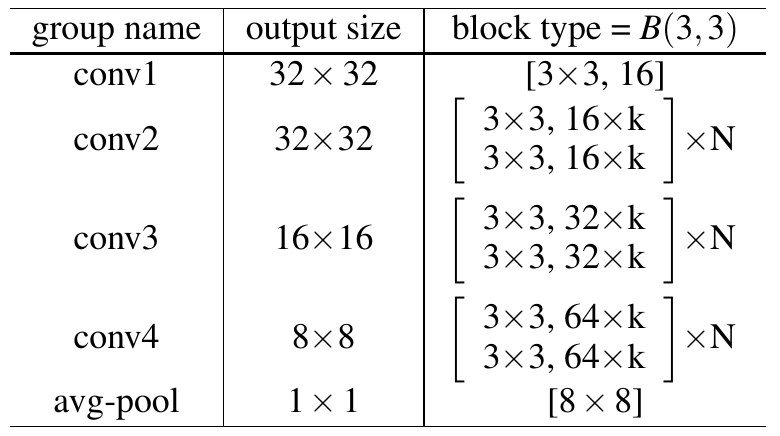
\includegraphics[width=0.49\linewidth]{images/wrn_block.png}
    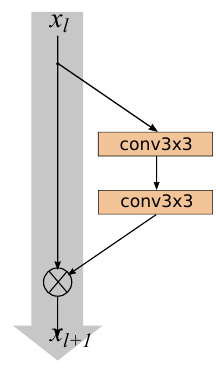
\includegraphics[width=0.165\linewidth]{images/block.png}
    \caption{General structure of a Wide Residual Network (left) and form of a single residual convolutional layer at each block, as presented in \cite{zagoruyko2016paying}. The factor $N$ which defines how many convolutional layers will be used at each block is not to be confused with the depth $n$ of the network, and is directly depended on $n$ via the formula $N =  (n - 4) \; div \;6 $.}
\end{figure}


\section{Generator Network}
\label{gen_lconfig}
The following table shows the layer structure of the generator network:

\begin{table}[h!]
    \centering
    \begin{tabular}{|c|c|c|c|}
    \toprule
    \toprule
    \textbf{\#Layer} & \textbf{Type} & \textbf{Configuration}\\
    \midrule
    1 & Linear & Input dim: 100, Output dim: 128*64\\
    \midrule
    2 & Batch Normalization & - \\
    \midrule
    3 & Upsampling & Scale factor: 2 \\
    \midrule
    4 & Convolutional & Input channels: 128, Output channels: 128\\
    \midrule
    5 & Batch Normalization & - \\
    \midrule
    6 & Activation & Leaky ReLU ($\alpha$ = 0.2)\\
    \midrule
    7 & Upsampling & Scale factor: 2 \\
    \midrule
    8 & Convolutional & Input channels: 128, Output channels: 64\\
    \midrule
    9 & Batch Normalization & - \\
    \midrule
    10 & Activation & Leaky ReLU ($\alpha$ = 0.2)\\
    \midrule
    11 & Convolutional & Input channels: 128, Output channels: 64\\
    \midrule
    12 & Batch Normalization & - \\
    \bottomrule
    \bottomrule
    \end{tabular}
    \caption{Layers of the generator network used in all zero-shot methods}
    \label{generator_layers}
    \end{table}
    
    For all the convolutional layers, the kernel size $k$ is equal to 3,while the stride $s$ and padding $p$ are equal to 1. 

\newpage
\section{Full Experiments}
\subsection{Training scratches of Wide ResNets}

In order to use Wide ResNets of different depth and width as teacher networks for the Few-Shot Attention Knowledge Distillation and the Zero-Shot Knowledge Transfer, we trained 4 variants of Wide ResNet from scratch. The results on CIFAR10 are shown in Table \ref{tab:scratch_cifar_10} below. 

\begin{table}[!h]
    \centering
    \begin{tabular}{c|ccc}
    \toprule
    \toprule
         \textbf{Model} & \textbf{Seed 0} & \textbf{Seed 1} & \textbf{Seed 2} \\
         \midrule
         WRN-16-1 & 90.97 & 91.41 & 91.78 \\
         WRN-16-2 & 94.21 & 94.27 & 94.18 \\
         WRN-40-1 & 93.52 & 94.04 & 93.94 \\
         WRN-40-2 & 95.14 & 95.12 & 95.23 \\
         \bottomrule 
         \bottomrule 
    \end{tabular}
    \vspace{0.25cm}
    \caption{Wide ResNet scratches performance on \textit{CIFAR-10}}
    \label{tab:scratch_cifar_10}
\end{table}

The results of training teachers on SVHN are shown in Table \ref{tab:scratch_svhn_10} below.  

\begin{table}[!h]
    \centering
    \begin{tabular}{c|ccc}
    \toprule
    \toprule
         \textbf{Model} & \textbf{Seed 0} & \textbf{Seed 1} & \textbf{Seed 2} \\
         \midrule
         WRN-16-1 & 95.52 & 95.43 & 95.47 \\
         WRN-16-2 & 96.17 & 96.09 & 96.03 \\
         WRN-40-1 & 96.07 & 96.14 & 96.19 \\
         WRN-40-2 & 96.14 & 96.13 & 96.37 \\
         \bottomrule
         \bottomrule
    \end{tabular}
    \vspace{0.25cm}
    \caption{Wide ResNet scratches performance on \textit{SVHN}}
    \label{tab:scratch_svhn_10}
\end{table}

\subsection{Training Wide ResNet 16-1 with no Teacher}

We also trained WRN-16-1 from scratch on small subsets of M images per class on CIFAR10 and SVHN and without the use of a teacher network to assist in the learning process. We firstly show the results on CIFAR10 in Table \ref{tab:few_show_cifar10_noteacher} below.

\begin{table}[!h]
    \centering
    \begin{tabular}{c|ccc}
    \toprule
    \toprule
         \textbf{M} & \textbf{Seed 0} & \textbf{Seed 1} & \textbf{Seed 2} \\
         \midrule
         10 & 23.7   & 21.68  & 25.86 \\
         25 & 34.4   & 38     & 36.07 \\
         50 & 41.69  & 44.2   & 45.27  \\
         75 & 54.45  & 51.89  & 50.99  \\
         100 & 57.02 & 56.87 & 56.69 \\
         \bottomrule
         \bottomrule
    \end{tabular}
    \vspace{0.25cm}
    \caption{Wide ResNet 16-1 few-shot training on \textit{CIFAR-10} with no assistance from a teacher network}
    \label{tab:few_show_cifar10_noteacher}

\end{table}

\newpage
The results on SVHN are the following in Table \ref{tab:few_show_svhn_noteacher}:

\begin{table}[!h]
    \centering
    \begin{tabular}{c|ccc}
    \toprule
    \toprule
         \textbf{M} & \textbf{Seed 0} & \textbf{Seed 1} & \textbf{Seed 2} \\
         \midrule
         10 & 11.97 & 12.67 & 11.73\\
         25 & 31.83 & 34.21 &  26.82\\
         50 & 44.08 & 45.93 & 42.93 \\
         75 & 50.07 & 41.88 & 53.96 \\
         100 & 56.71 & 69.58 & 59.56 \\
         200 & 87.65 & 87.92 & 87.18\\
         \bottomrule
         \bottomrule
    \end{tabular}
    \vspace{0.25cm}
    \caption{Wide ResNet 16-1 few-shot training on \textit{SVHN} with no assistance from a teacher network}
    \label{tab:few_show_svhn_noteacher}

\end{table}

\subsection{Few-Shot Knowledge Distillation with Attention Transfer (KD-AT)}

Few-Shot Knowledge Distillation with Attention Transfer is trained using different pairs of Teacher-Student and different values of M for CIFAR-10 and SVHN datasets. We firstly show the results on CIFAR10 using WRN-40-2 for the Teacher and WRN-16-1 for the Teacher, for different values of M in Table \ref{tab:few_show_cifar10_mvalues}.

\begin{table}[!h]
    \centering
    \begin{tabular}{c|ccc}
    \toprule
    \toprule
         \textbf{M} & \textbf{Seed 0} & \textbf{Seed 1} & \textbf{Seed 2} \\
         \midrule
         10 & 39.08 & 35.33 & 36.49\\
         25 & 60.05 & 58.94 & 63.05\\
         50 & 70.9 & 65.83 & 68.68\\
         75 & 73.84 & 74.29 & 77\\
         100 & 76.67 & 76.72 & 79.57\\
         5000 & 92.15 & 92.25 & 92.17  \\
         \bottomrule
         \bottomrule
    \end{tabular}
    \vspace{0.25cm}
    \caption{Few-shot training on \textit{CIFAR-10} with Attention Transfer using WRN-40-2 for the Teacher and WRN-16-1 for the Student, for different values of M}
    \label{tab:few_show_cifar10_mvalues}

\end{table}

The results on SVHN using WRN-40-2 for the Teacher and WRN-16-1 for the Student, for different values of M are shown in Table \ref{tab:few_show_svhn_mvalues}.

\begin{table}[!h]
    \centering
    \begin{tabular}{c|ccc}
    \toprule
    \toprule
         \textbf{M} & \textbf{Seed 0} & \textbf{Seed 1} & \textbf{Seed 2} \\
         \midrule
         10 & 37.35 & 31.32 & 33.88\\
         25 & 48.71 & 48.89 & 47.44\\
         50 & 68.84 & 65.33 & 66.48\\
         75 & 78.51 & 78.4 &  79.28\\
         100 & 81.18 & 79.63 & 81.45 \\
         5000 & 95.19 & 95.44 & 95.72 \\
         \bottomrule
         \bottomrule
    \end{tabular}
    \vspace{0.25cm}
    \caption{Few-shot training on \textit{SVHN} with Attention Transfer using WRN-40-2 for the Teacher and WRN-16-1 for the Student, for different values of M}
    \label{tab:few_show_svhn_mvalues}
\end{table}

\newpage
The results for different pairs of Teacher-Student for M=200 is shown in Table \ref{tab:few_cifar_m_200}. 

\begin{table}[!h]
    \centering
    \begin{tabular}{cc|ccc}
    \toprule
    \toprule
         \textbf{Teacher} & \textbf{Student} & \textbf{Seed 0} & \textbf{Seed 1} & \textbf{Seed 2} \\
         \midrule
         WRN-16-2 & WRN-16-1 & 85.51 & 85.26 & 85.89 \\
         WRN-40-1 & WRN-16-1 & 83.9 & 83.35 & 83.67 \\
         WRN-40-1 & WRN-16-2 & 87.52 & 87.14 & 87.13 \\
         WRN-40-2 & WRN-16-1 & 82.41 & 81.97 & 84.18 \\
         WRN-40-2 & WRN-16-2 & 87.15 & 86.49 & 88.18\\
         WRN-40-2 & WRN-40-1 & 88.18 & 87.77 & 89.29 \\
         \bottomrule
         \bottomrule
    \end{tabular}
    \vspace{0.25cm}
    \caption{Teacher-Student Wide ResNets few-shot training on CIFAR-10 with Attention Transfer, for \textit{M = 200}}
    \label{tab:few_cifar_m_200}
\end{table}

\subsection{Zero-Shot Knowledge Transfer}

We trained the zero-show Knowledge transfer algorithm for various pairs of Teacher Student for CIFAR-10 and SVHN. In Table \ref{tab:zero_shot_cifar_10} the results for CIFAR-10 is shown for various seeds and Teacher Student pairs and in Table \ref{tab:zero_shot_svhn} the experiment for SVHN is shown.

\begin{table}[!h]
    \centering
    \begin{tabular}{cc|ccc}
    \toprule
    \toprule
         \textbf{Teacher} & \textbf{Student} & \textbf{Seed 0} & \textbf{Seed 1} & \textbf{Seed 2} \\
         \midrule
         WRN-16-2 & WRN-16-1 & 80.59 & 80.7 & 82.48 \\
         WRN-40-1 & WRN-16-1 & 77.4 & 80.61 & 81.7 \\
         WRN-40-1 & WRN-16-2 & 88.71 & 87.34 & 87.08 \\
         WRN-40-2 & WRN-16-1 & 83.73 & 83.76 & 83.42 \\
         WRN-40-2 & WRN-16-2 & 89.13 & 89.48 & 89.32\\ 
         WRN-40-2 & WRN-40-1 & 87.94 & 87.28 & 87.18  \\
         \bottomrule
         \bottomrule
    \end{tabular}
    \vspace{0.25cm}
    \caption{Teacher-Student Wide ResNets zero-shot training on \textit{CIFAR-10}}
    \label{tab:zero_shot_cifar_10}

\end{table}


\begin{table}[!h]
    \centering
    \begin{tabular}{cc|ccc}
    \toprule
    \toprule
         \textbf{Teacher} & \textbf{Student} & \textbf{Seed 0} & \textbf{Seed 1} & \textbf{Seed 2} \\
         \midrule
         WRN-40-2 & WRN-16-1 & 94.21 & 93.85 & 93.94 \\
         \bottomrule
         \bottomrule
    \end{tabular}
    \vspace{0.25cm}
    \caption{Teacher-Student Wide ResNets zero-shot training on \textit{SVHN}}
    \label{tab:zero_shot_svhn}

\end{table}


\subsection{Zero-Shot Knowledge Transfer with modified generator}

Table \ref{tab:zeroShot_modified} shows the results for the modified zero-shot we tried.


\begin{table}[!h]
    \centering
    \begin{tabular}{cc|ccc}
    \toprule
    \toprule
         \textbf{Teacher} & \textbf{Student} & \textbf{Seed 0} & \textbf{Seed 1} & \textbf{Seed 2} \\
         \midrule
         WRN-16-2 & WRN-16-1 & 82.42 & 81.73 & 84.32 \\
         WRN-40-1 & WRN-16-1 & 79.87 & 84.62 & 83.34\\
         WRN-40-1 & WRN-16-2 & 88.71 & 90.11 & 88.99 \\
         WRN-40-2 & WRN-16-1 & 85.09 & 84.07 & 85.18 \\
         WRN-40-2 & WRN-16-2 & 90.67 & 91.41 & 91.27 \\ 
         WRN-40-2 & WRN-40-1 & 90.08 & 90.16 & 90.59 \\
         \bottomrule
         \bottomrule
    \end{tabular}
    \vspace{0.25cm}
    \caption{Teacher-Student Wide ResNets zero-shot training on \textit{CIFAR-10} with \textit{modified generator}}
    \label{tab:zeroShot_modified}

\end{table}
\newpage
\subsection{Zero-Shot Knowledge Transfer with extra M real samples}

Our results in CIFAR10 when extra samples are drawn from the generator, are presented in Table \ref{tab:zeroShot_KDatt_cifar}.

\begin{table}[!h]
    \centering
    \begin{tabular}{c|ccc}
    \toprule
    \toprule
         \textbf{M} & \textbf{Seed 0} & \textbf{Seed 1} & \textbf{Seed 2} \\
         \midrule
         10 & 83.89 & 83.37 & 83.77 \\
         25 & 84.08 & 83.57 & 84.22 \\
         50 & 84.69 & 84.37 & 84.94 \\
         75 & 84.98 & 84.53 & 85.0  \\
         100 & 85.27 & 84.73 & 85.35\\
         \bottomrule
         \bottomrule
    \end{tabular}
    \vspace{0.25cm}
    \caption{Performance of Zero-Shot pre-trained student WRN-16-1 when few-shot knowledge distillation is performed from a teacher WRN-40-2 for a few epochs with M samples.}
    \label{tab:zeroShot_KDatt_cifar}
\end{table}

The same setting is repeated on the SVHN dataset in Table \ref{tab:zeroShot_KDatt_svhn} with the following results:

\begin{table}[!h]
    \centering
    \begin{tabular}{c|ccc}
    \toprule
    \toprule
         \textbf{M} & \textbf{Seed 0} & \textbf{Seed 1} & \textbf{Seed 2} \\
         \midrule
         10 & 94.29 & 93.9 & 94.0   \\
         25 & 94.26 & 93.97 & 93.98 \\
         50 & 94.26 & 93.94 & 93.97 \\
         75 & 94.27 & 93.95 & 93.94 \\
         100 & 94.24 & 93.97 & 93.94 \\
         \bottomrule
         \bottomrule
    \end{tabular}
    \vspace{0.25cm}
    \caption{Performance of Zero-Shot pre-trained student WRN-16-1 when few-shot knowledge distillation is performed from a teacher WRN-40-2 for a few epochs with M samples.}
    \label{tab:zeroShot_KDatt_svhn}
\end{table}

\subsection{Modified Zero-Shot Knowledge Transfer with extra M real samples}

Our results in CIFAR10 when extra samples are drawn from the generator, are presented in Table \ref{tab:modified_zeroShot_KDatt_cifar}.

\begin{table}[!h]
    \centering
    \begin{tabular}{c|ccc}
    \toprule
    \toprule
         \textbf{M} & \textbf{Seed 0} & \textbf{Seed 1} & \textbf{Seed 2} \\
         \midrule
         10 & 85.09 & 84.54 & 85.31 \\
         25 & 85.09 & 85.21 & 85.43 \\
         50 & 86.37 & 86.18 & 86.29 \\
         75 & 86.77 & 86.4  & 86.67 \\
         100 & 87.2 & 86.74 & 86.96\\
         \bottomrule
         \bottomrule
    \end{tabular}
    \vspace{0.25cm}
    \caption{Performance of Zero-Shot pre-trained student WRN-16-1 when few-shot knowledge distillation is performed on top of our modified training method from a teacher WRN-40-2 for a few epochs with M samples.}
    \label{tab:modified_zeroShot_KDatt_cifar}
\end{table}

\newpage
\section{Samples for Measuring Belief Matching}

The following figure shows the evolution of images when manipulated at different steps regarding the belief matching experiment conducted in section 4.5:

\begin{figure}[H]
   \centering
   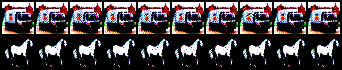
\includegraphics[width=120mm]{images/KD-sample2-class97.png}
   \caption{Two test samples from the measuring of belief matching. The figure shows the original images and the result of $K=100$ altering steps towards each other class.}
  \label{manipulateSamples}
\end{figure}

\section{Transition Curves of Teacher Updates}

\begin{figure}[H]
   \centering
   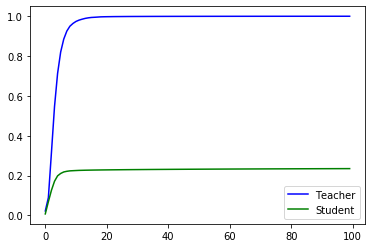
\includegraphics[width=.45\linewidth]{images/KD-AT-Teacher-Train.png}
   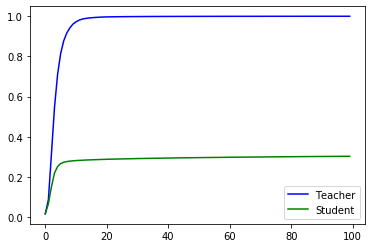
\includegraphics[width=.45\linewidth]{images/Zero-Shot-Teacher-Train.png}
   \caption{Transition curves of teacher and student with KD-AT (left) and Zero-Shot (right) methods when sample are updated based on the gradients of the teacher.}
\end{figure}
